\title{Self Organizing Systems Exercise 2}
\author{
        Alexander Dobler 01631858\\
        Thomas Kaufmann 01129115 
}
\date{\today}

\documentclass[12pt]{article}

\usepackage{hyperref}
\usepackage{booktabs}
\usepackage{graphics}
\usepackage{multirow}
\usepackage{graphicx}
\usepackage{subcaption}
\usepackage{mwe}
\usepackage{amsmath,amssymb}
\usepackage{subcaption}

\begin{document}
\maketitle

\begin{abstract}
    In the second exercise of the lecture Self Organizing Systems we are implementing a simple Particle Swarm Optimization (PSO) algorithm and experimenting with different parameters, fitness functions, constraints and constraint handling method.
    More specifically, we are given a PSO framework in NetLogo for optimizing functions $f$ from $\mathbb{R}^2$ to $\mathbb{R}$.
    Our task is to implement 3 different fitness functions, 3 different constraints and a constraint handling method using penalization.
    Furthermore, we are to conduct several experiments, to observe different effects of parameters on the performance of the convergence behaviour of the PSO algorithm.
    Here we are inspecting \textit{population size}, \textit{particle speed limit}, \textit{particle inertia} and the difference between constraint handling using penalization and rejection.
\end{abstract}

\section{Implementation}
In this section we will describe how we implemented the required tasks given in the exercise.
We will divide this section into explanations for \textit{constraints}, \textit{fitness functions} and \textit{constraint handling with penalization}.

\subsection{Constraints}
As we are already given skeletons for constraints, implementing is as easy as returning \textit{true}, if the constraint is violated and \textit{false} otherwise.
We opted for implementing the following constraints.
\begin{enumerate}
        \item $x^2+y^2<6000$
        \item $x^2+y^2<9000\text{ and }x^2+y^2>4000$
        \item $\tan(2x)<\tan(4y)$
\end{enumerate}
So, if for example for the first constraint it holds that $x^2+y^2>=6000$, the constraint is violated and we return true.
We selected these constraints, as we wanted to have functions with one connected region (constraint 1 and 2) and also constraints with miltiple separated regions (constraint 3).
\subsection{Fitness Functions}
Here we have a similar setting as for constraints, because we already have skeletons for fitness functions.
We opted to implement the following functions.
\begin{enumerate}
        \item Schaffer function
        \item Booth's function
        \item Schwefel function
\end{enumerate}
Scaling $x$ and $y$ variables for the input of the functions is done as already shown in the template.
It is also important to mention that the NetLogo $\sin$-function expects angles in degrees as input, so we had to convert radians to degrees first.
For the Schwefel function we had to set $n:=2$ and $x_1=x,x_2=y$ for our purpose of two dimensions.

We chose these functions as we wanted to have both optima at the corners of the grid and optima in the middle of the grid.
Furthermore we also have a diversity of how many local optima the search-space of the different functions have.
\subsection{Constraint Handling with Penalization}
The implementation for penalization is more interesting.
First we created 4 different functions to calculate penalization values for each constraint (the example constraint included).
So for each constraint we can compute its penalty value at patch $x,y\in\mathbb{R}^2$, if the constraint is violated at this patch.
This penalty value is $C(x,y)\cdot d$ for constraints $C(x,y)<0$ and a constant $d$.
For example for constraint 1 we have $(x^2+y^2-6000)\cdot d$ as penalty value if $x^2+y^2\ge 6000$.
Furthermore we wanted penalty values to be between 0 and 1, so we chose constants $d$ appropriately.
So for example for constraint 1 we set $d:=\frac{1}{14000}$ as $C(x,y)=x^2+y^2-6000$ can be as big as $14000$ for $x=y=100$.

We then add these penalty values at position $(x,y)$ to the value of the patch at position $(x,y)$ if the selected contraint is violated at position $(x,y)$.
This, of course, is only done if penalization is selected as constraint handling method.
Due to this variant of implementation, we do not have to update anything in the \textit{update-particle-positions}, as fitness-functions at patches are already considering penalization by the selected constraint.


\section{Experiments and Analysis}
\subsection{Experimental Setup \& Evaluation Metrics}
In order to compare the convergence behaviour, we use a fixed number of up to $200$ iterations, without any time limit. 
Furthermore, we disabled the premature termination criterion once the optimum is found, since this would have led to bias results in our stepwise average approach. 

We use the following metrics to capture characteristics of solutions:
\begin{itemize}
	\item \textbf{Fitness}: a value between 0 and 1
	\item \textbf{Number of Clusters}: To get a feeling of the distribution of particles in the search space.
	We use the clustering algorithm of the netlogo plugin \emph{dbscan}, where a cluster is constituted of at least three agents with a maximum distance of $5$. 
	These values have been selected manually based on some manual tweaking and tuning. 
	
	\begin{figure}[h!]
		\centering
			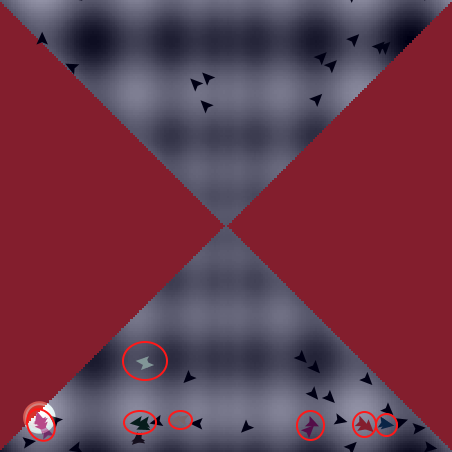
\includegraphics[width=5cm]{figures/clusters.png}
			\caption{Illustration of Clusters in a constrained Schwefel Function Optimization Instance.}
			\label{fig:clusters}
	\end{figure}	

	Figure~\ref{fig:clusters} illustrates a few clusters in an early iteration in a Schaffer optimization instance. 
	With this metric, in combination with others, we aim to identify scenarios where agents split up into separate groups, converging towards different regions in the search space. 
	We normalized the number of clusters by the population size, to foster comparability in plots. 
	
	
	\item \textbf{Average Distance to the Optimal Solution}: Should be monotonically decreasing in convex functions. However, in rugged landscapes with several nearly optimal solutions may not necessarily decrease to $\approx 0$.
	\item \textbf{Average Distance among Particles}: As a measure for the distribution of particles in the search space. 
	Thus, in the beginning it is relatively high, as particles are randomly scattered among the search space, but it should decrease continuously as particles strive towards the (single or few) global optima. 
	In case this value is high, a disconnected and highly constrained search may be indicated. 
	\item \textbf{Average Path Length}: Average length of the paths of each particle throughout the entire execution.
		
\end{itemize}

Finally, for statistically stable results, each configuration in our experiments was executed $15$ times, and metrics where obtained by the average of those executions.
%\subsection{Experiment 1: Strong Personal Focus}
%\begin{figure}
%	\centering
%	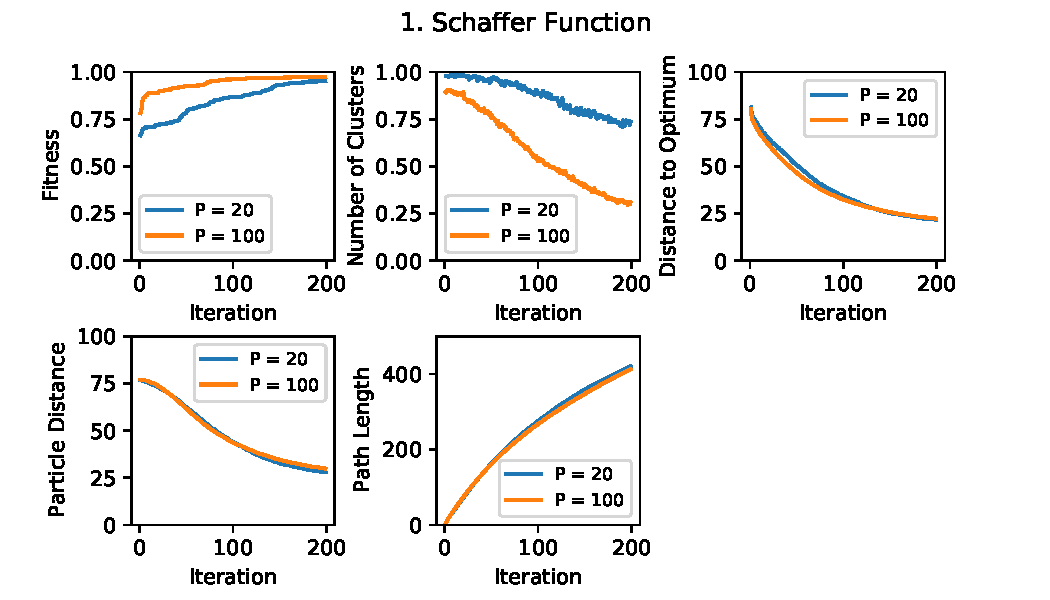
\includegraphics[width=0.75\textwidth]{figures/ex1/ex1-1.pdf}
%	\label{fig:ex1-1}
%\end{figure}
%\begin{figure}
%	\centering
%	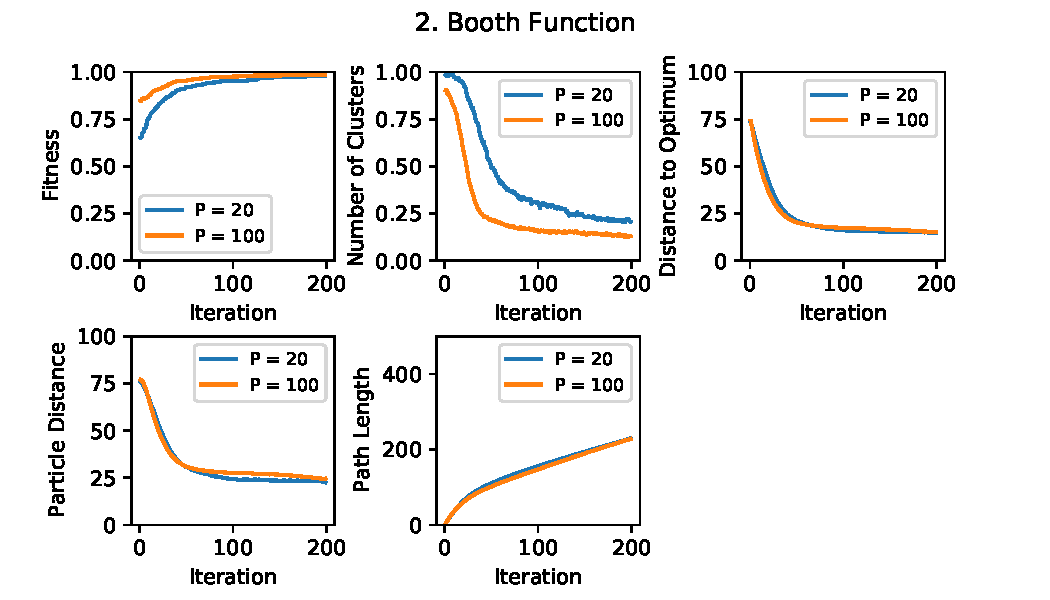
\includegraphics[width=0.75\textwidth]{figures/ex1/ex1-2.pdf}
%	\label{fig:ex1-2}
%\end{figure}
%
%\begin{figure}
%	\centering
%	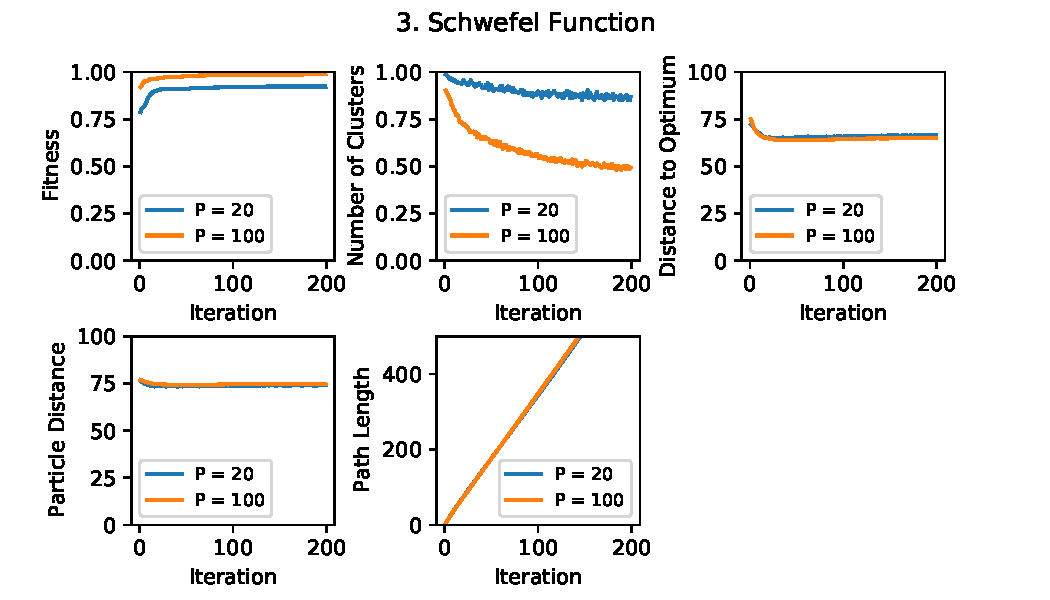
\includegraphics[width=0.75\textwidth]{figures/ex1/ex1-3.pdf}
%	\label{fig:ex1-3}
%\end{figure}
%strong personal focus and scarce distribution in the beginning, hard to find neighbour that guides somewhere
%in easier functions even small population sizes 
%\begin{figure}
%\begin{subfigure}[c]{0.5\textwidth}
%\centering
%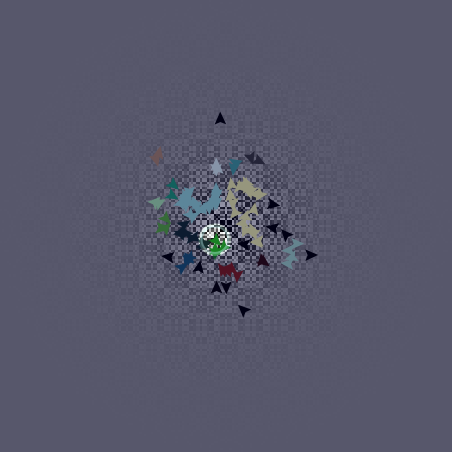
\includegraphics[width=0.75\textwidth]{figures/ex1/f1.png}
%\subcaption{F1}
%\end{subfigure}
%\begin{subfigure}[c]{0.5\textwidth}
%\centering
%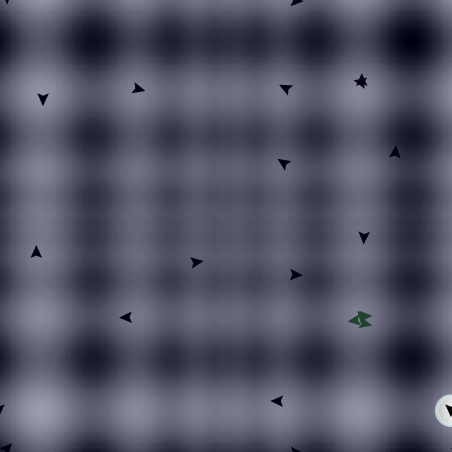
\includegraphics[width=0.75\textwidth]{figures/ex1/f3.png}
%\subcaption{F3}
%\end{subfigure}
%
%\caption{Comparison of representative solutions for fitness function $1$ ($P=100$) and $3$ ($P=20$).}
%
%\end{figure}

\subsection{Different Population Sizes}
In the first experiment we compare the impact of the population size on the convergence behaviour. 
For each function, we compared three different population sizes with fixed parameters for the others (inertia $\omega=0.33$, swarm-confidence $c_s=1$, personal-confidence $c_p=1$ and particle-speed-limit $V_{max}=10$).
Observations based on Figures~\ref{fig:ex2-1},\ref{fig:ex2-2},\ref{fig:ex2-3}:
\begin{itemize}
	\item Larger populations are in favour of finding the global optimum or at least converge faster. 
	One reason for this is certainly the relatively restricted search space, where it's rather likely that a random initialization hits high quality regions right in the beginning. 
	We conducted some small experiments with completely unsuitable parameter settings, but large populations that still obtained the global optimum in just a couple of iterations. 
	\item For extraordinarily small populations, e.g. $P=10$, the experiments show that only for rather simple functions without a rugged landscape convergence towards the optimum can be achieved (Booth's function seems to be \emph{convexish}, although it is quadratic). 
	\item For more complex functions, like Schaffer, those populations converge at several poor local optima around the global one, indicated by the relatively high number of different clusters and the high average distance to the optimum. 
	Still, after $30$ iterations they seem to concentrate on a certain subspace, where they get stuck in local optima. 
	\item Although convergence towards a suboptimal solution w.r.t to the fitness sets in rather early, the path lengths still increases, indicating stagnation behaviour. 
\end{itemize}

\begin{figure}[h!]
	\centering
	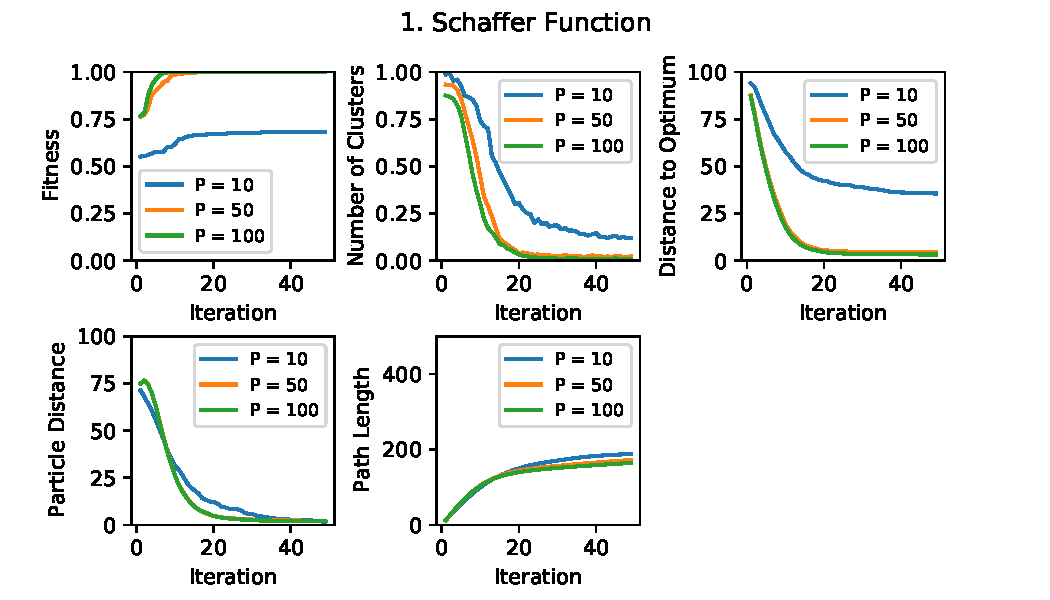
\includegraphics[width=0.75\textwidth]{figures/ex2/ex2-1.pdf}
	\caption{Metrics for Schaffer Function}
	\label{fig:ex2-1}
\end{figure}
\begin{figure}[h!]
	\centering
	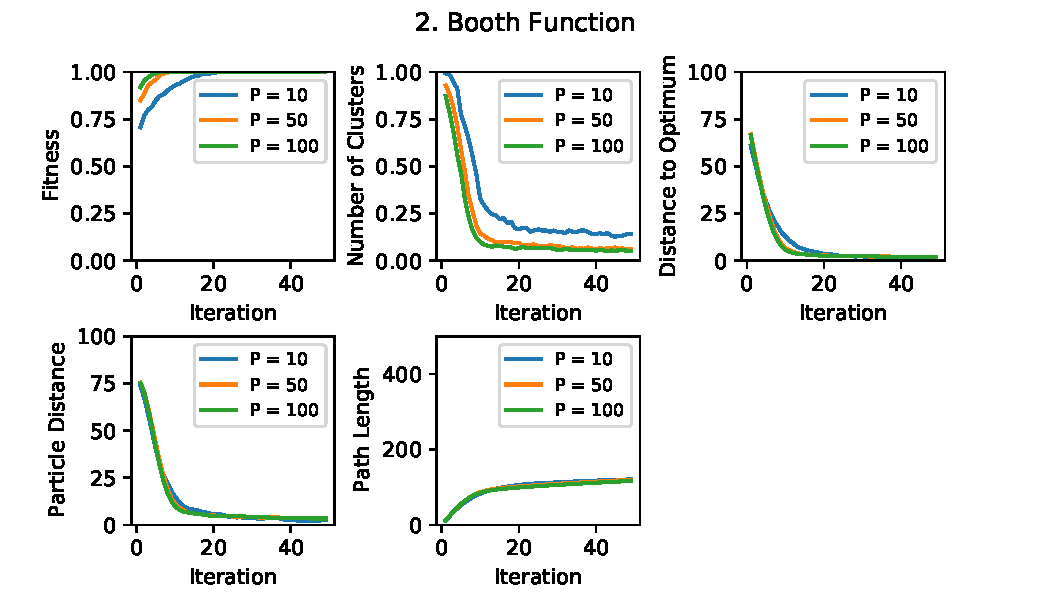
\includegraphics[width=0.75\textwidth]{figures/ex2/ex2-2.pdf}
	\caption{Metrics for Booth Function}
	\label{fig:ex2-2}
\end{figure}
\begin{figure}[h!]
	\centering
	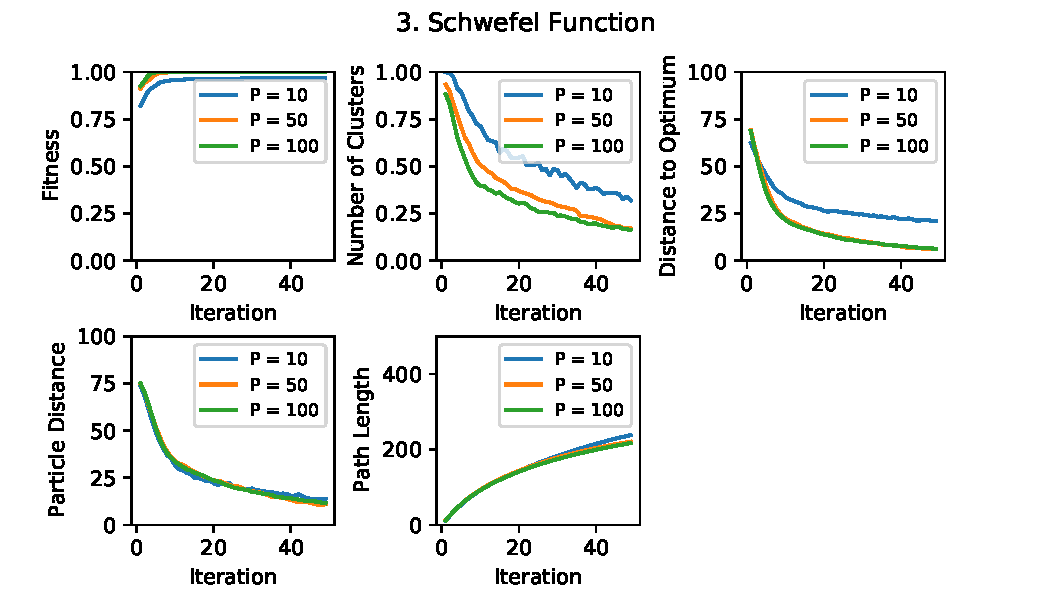
\includegraphics[width=0.75\textwidth]{figures/ex2/ex2-3.pdf}
	\caption{Metrics for Schwefel Function}
	\label{fig:ex2-3}
\end{figure}


\subsection{Acceleration Coefficients}
Based on our findings we proceeded with experiments concerning acceleration coefficients. 
From manual tests and the previous experiment, we know that for larger populations our functions can be optimized quite easily with standard parameters, $c_s=1$, $c_p=1$ and $V_{max}=10$, so in this experiment we turned our focus on values off the mean (i.e. $1$) and tested all four combinations for the values $0.3$ and $1.7$ for medium and larger population sizes for each of the selected functions. 

Observations based on Figures~\ref{fig:ex4-1-20},\ref{fig:ex4-1-50},\ref{fig:ex4-2-20},\ref{fig:ex4-2-50},\ref{fig:ex4-3-20},\ref{fig:ex4-3-50}:
\begin{itemize}
	\item Our main observation from this experiment was that in the selected functions, a dominance of swarm-confidence is favourable in terms of convergence. 
	Even for smaller populations convergence towards a high quality optimum can be obtained even below $20$ iterations.
	\item Even further, the number of particles temporarily stuck in suboptimal local seems to be lower, indicated by our cluster metric, which in combination with the distance to the global optimum, shows a relatively smooth convergence in just $20$ iterations. 
	\item For other configurations, on the other hand, these metrics show a different picture. 
	First, there's a lot of fluctuations in the number of clusters, indicating that particles frequently change influencing neighbours, although eventually they still converge towards the optimum on average (but with far more particles being in many other regions in the search space). 
	It is important to note that this is actually not necessarily a poor characteristic. 
	For other functions, particularly with larger and potentially more rugged search spaces, we claim that such a behaviour is actually to some degree advantageous since it fosters diversity in the search (still it perfectly shows that parameters highly depend on the instance).
	\item For the inverse dominance relationship between swarm and personal confidence a rather poor behaviour can be observed. 
	First, this configuration lacks in convergence towards the optimum w.r.t to fitness, but also the other metrics show poor behaviour. 
	Throughout the entire search, the number of distinct clusters remains relatively high, indicating that particles likely do not profit from each other, but rather seem to be stuck in intensifications phases (the path length is still relatively high, indicating that particles still make significant steps but without any real progress in terms of fitness, also shown by the high average distance to the optimum). 
	\item Figure~\ref{fig:ex4-example} shows two representative examples of this behaviour. 
	On the one hand, ~\ref{fig:ex4-example-a} shows almost arbitrarily scattered particles in the search space after $100$ iterations, while in ~\ref{fig:ex4-example-b} all particles were directly guided towards the optimum. 
	\item Again, it can be observed that Booth's function is among the easier ones, where even poor configurations obtain the optimum relatively fast. 
\end{itemize}




\begin{figure}[h!]
	\centering
	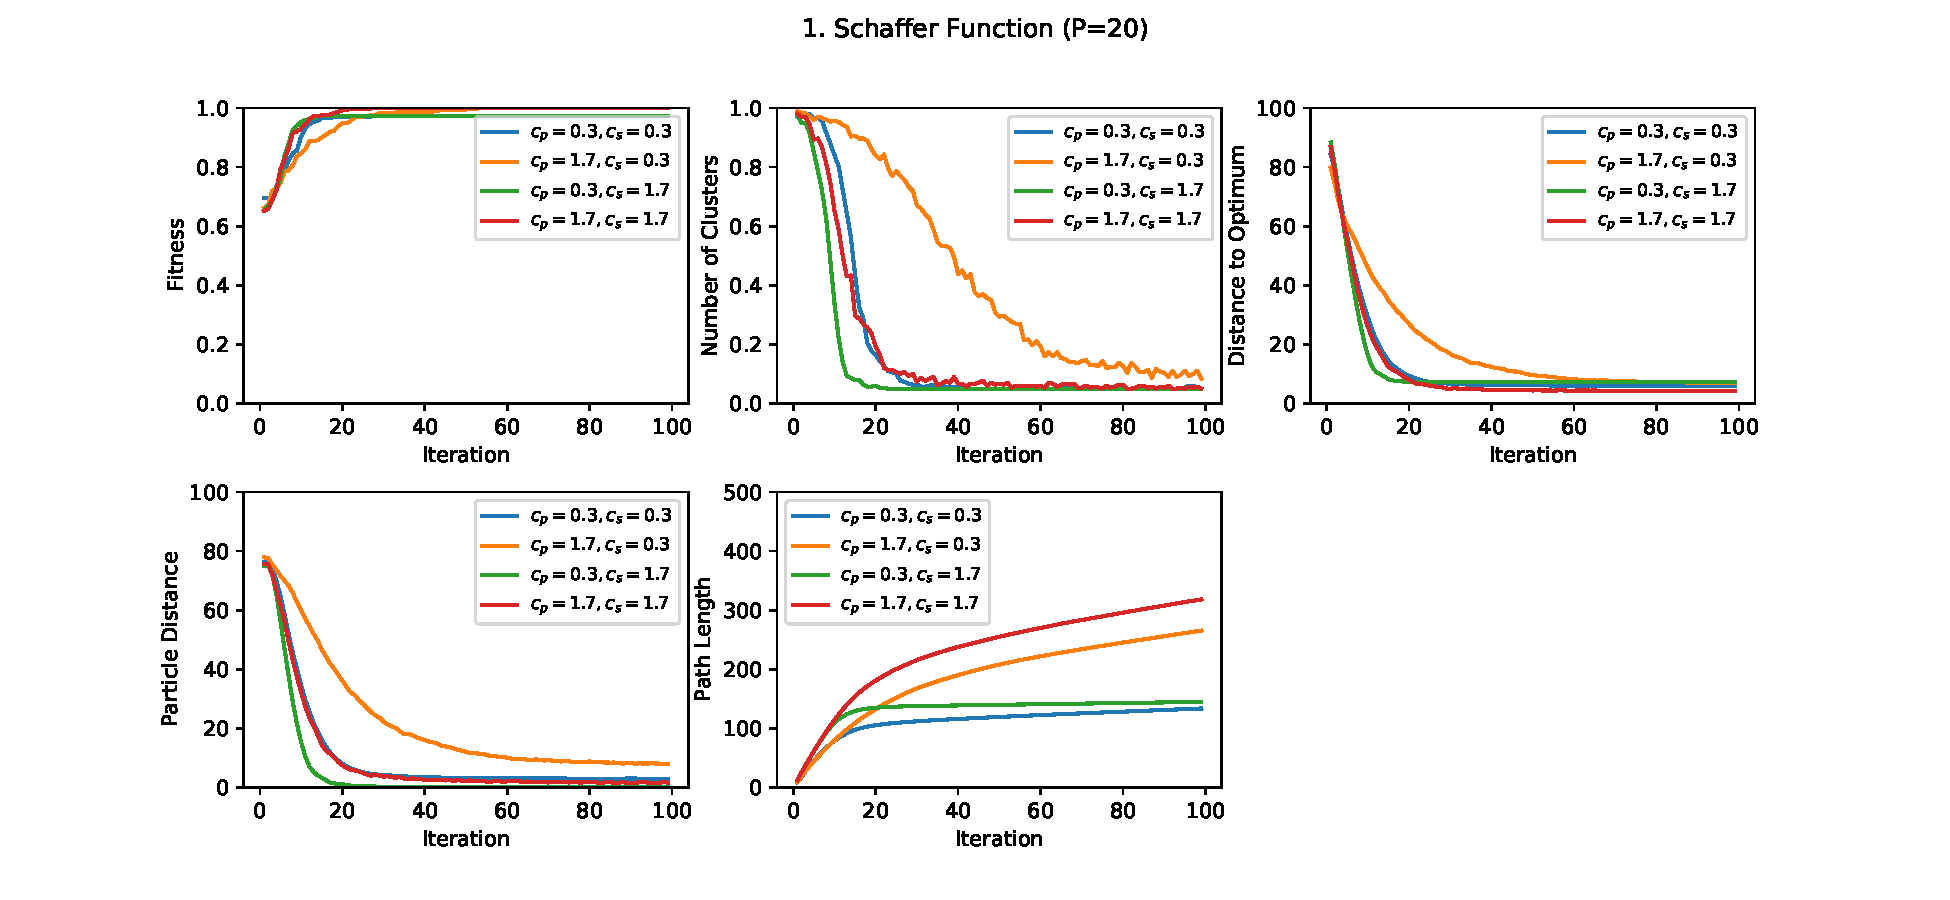
\includegraphics[width=1\textwidth]{figures/ex4/ex4-1-20.pdf}
	\caption{Metrics for Schaffer function and $P=20$}
	\label{fig:ex4-1-20}
\end{figure}
\begin{figure}[h!]
	\centering
	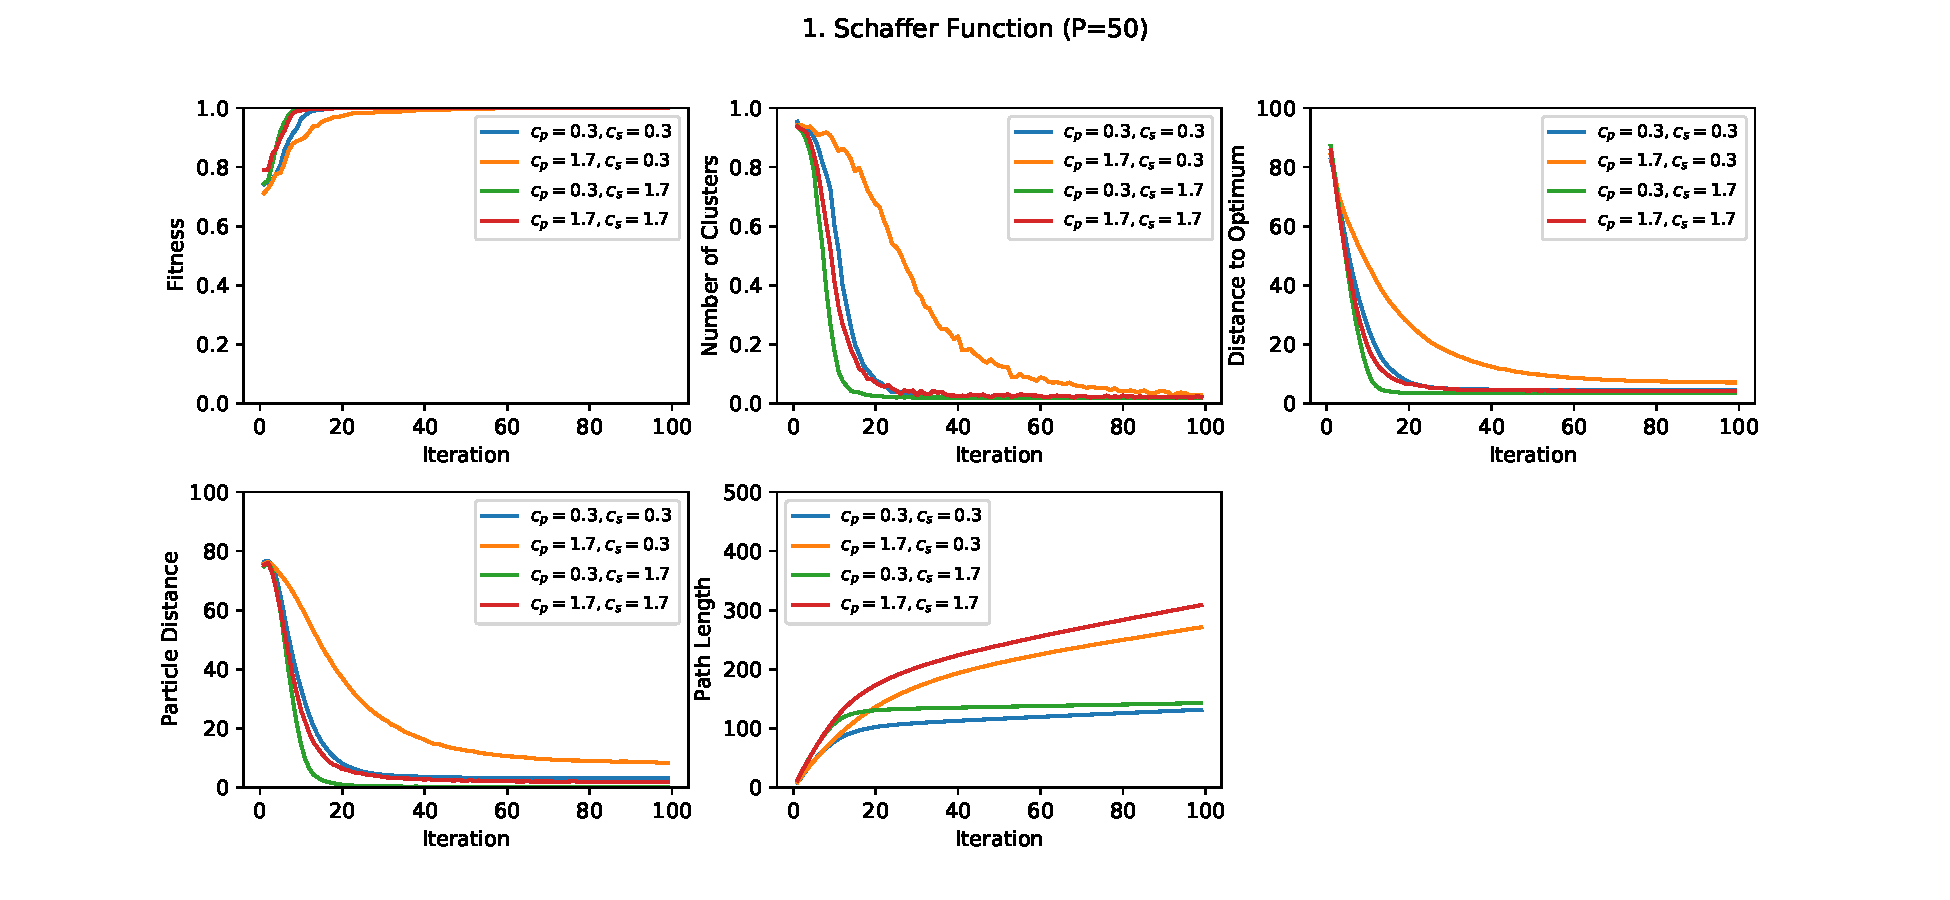
\includegraphics[width=1\textwidth]{figures/ex4/ex4-1-50.pdf}
	\caption{Metrics for Schaffer function and $P=50$}
	\label{fig:ex4-1-50}
\end{figure}
\begin{figure}[h!]
	\centering
	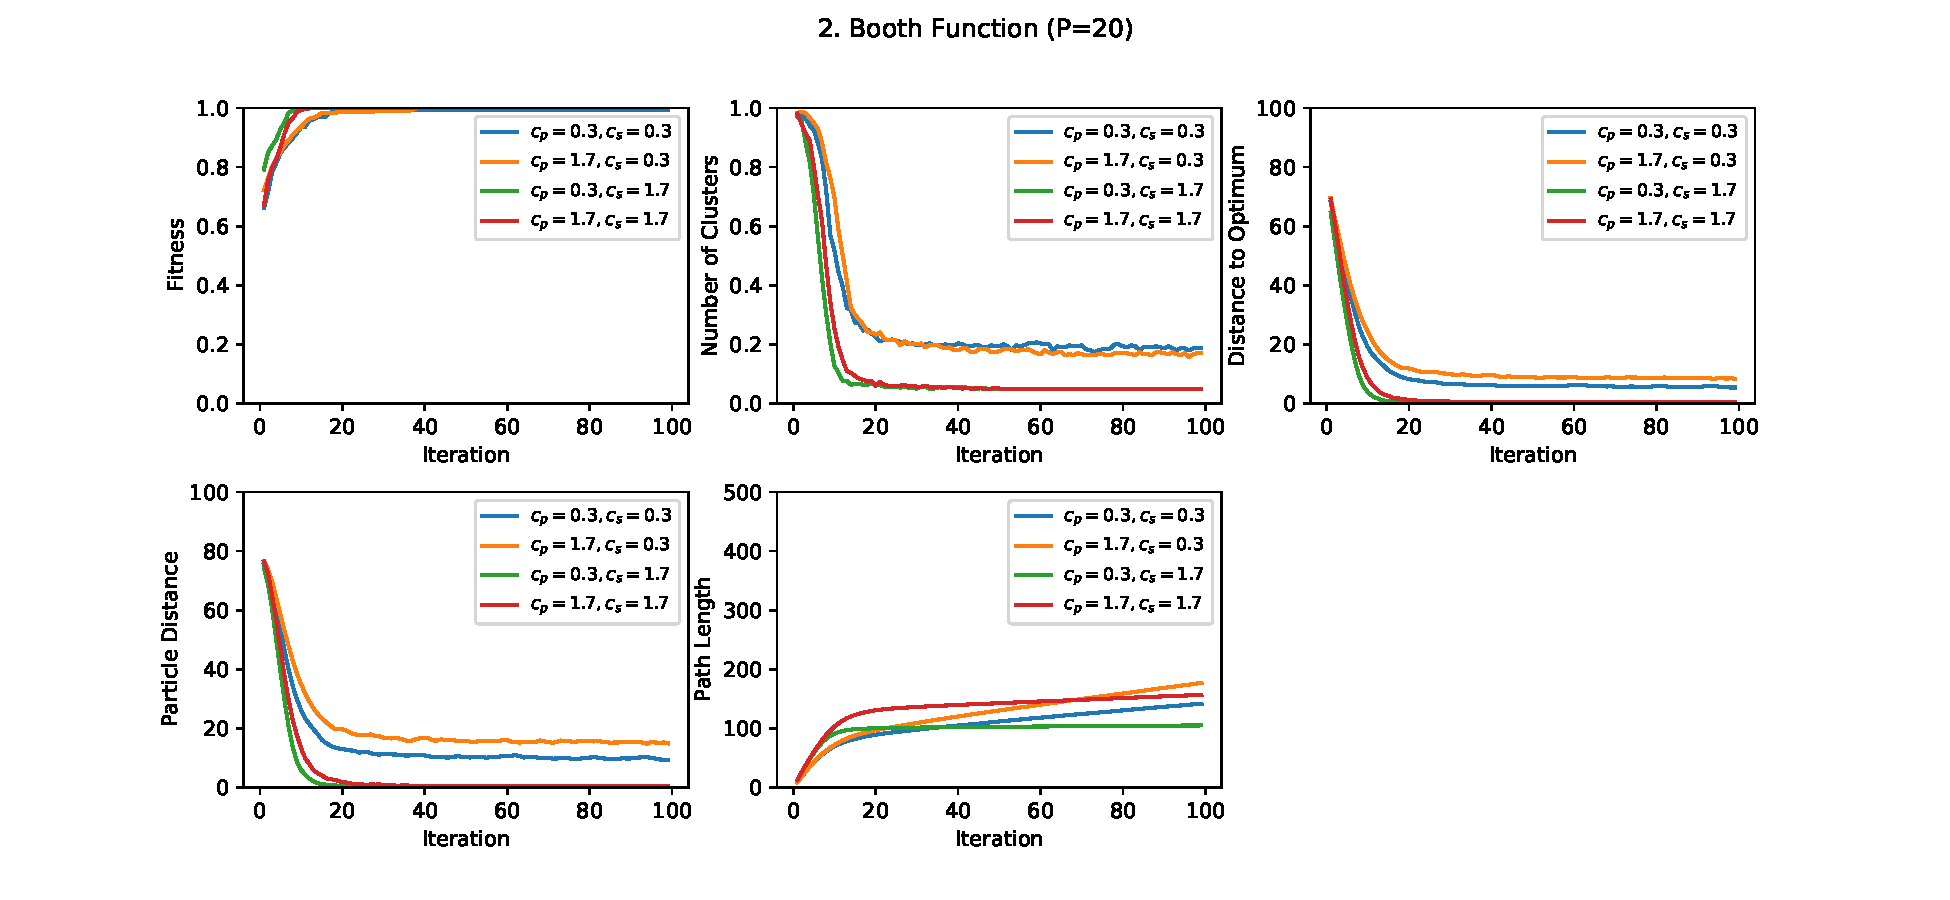
\includegraphics[width=1\textwidth]{figures/ex4/ex4-2-20.pdf}
	\caption{Metrics for Booth function and $P=20$}
	\label{fig:ex4-2-20}
\end{figure}
\begin{figure}[h!]
	\centering
	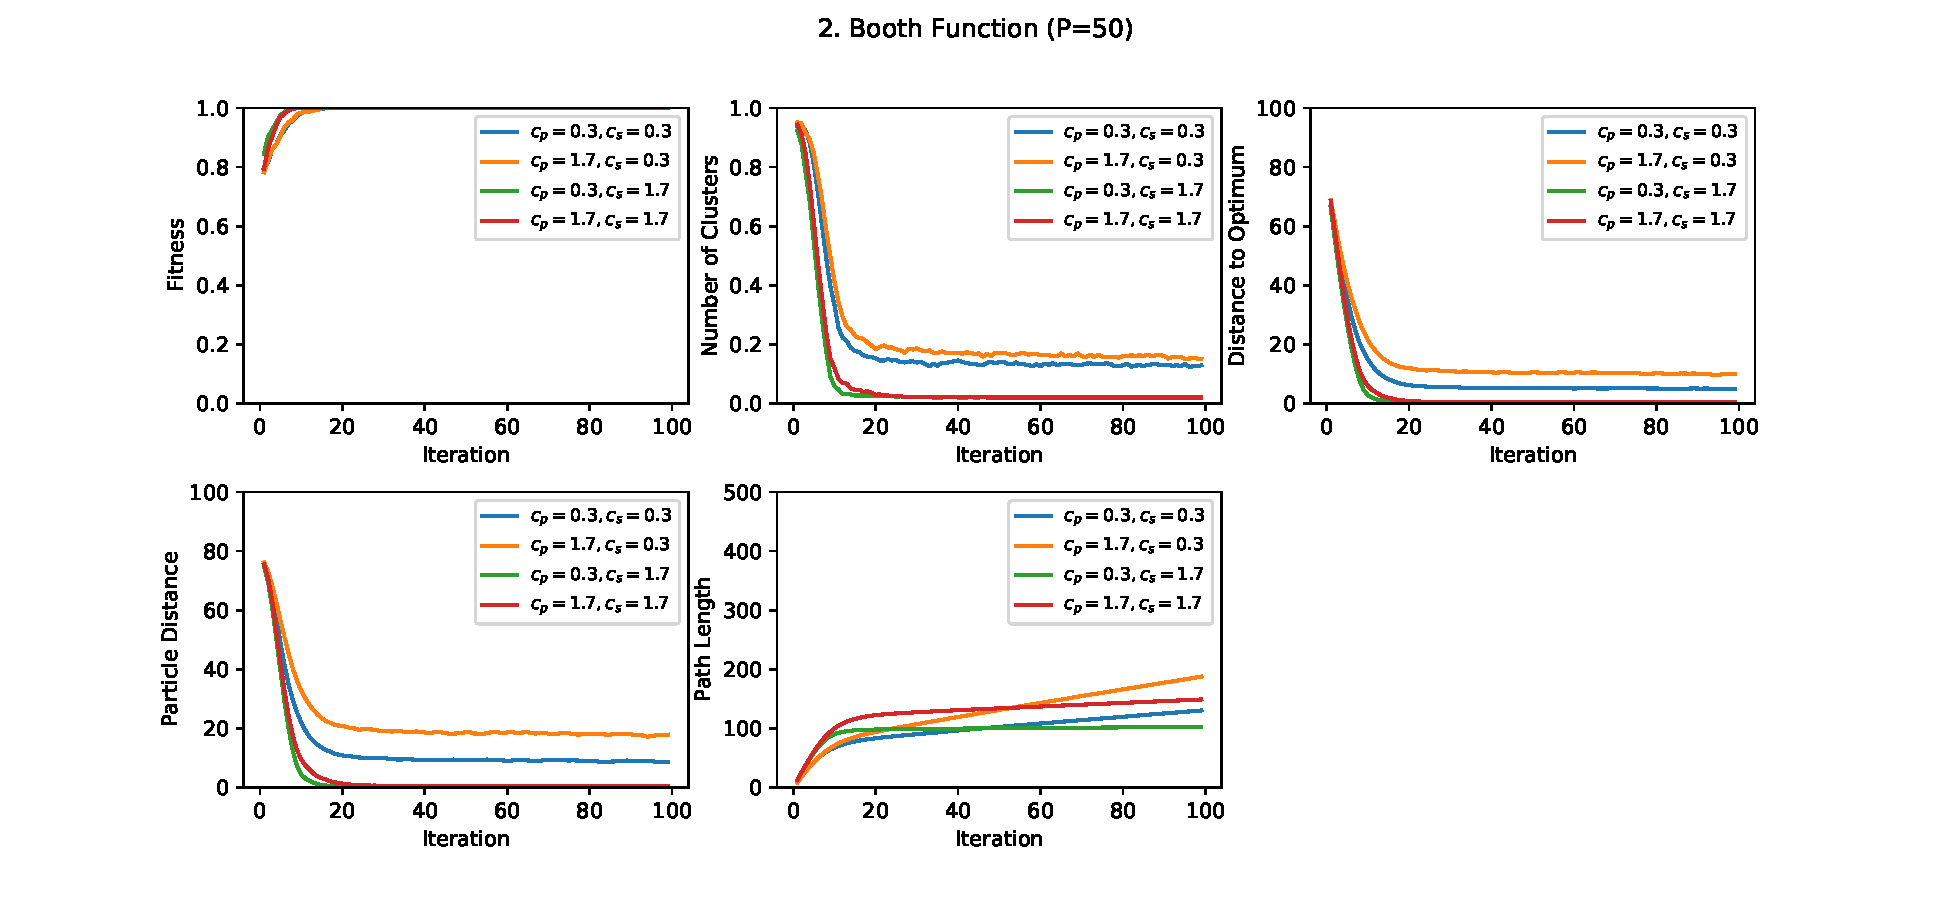
\includegraphics[width=1\textwidth]{figures/ex4/ex4-2-50.pdf}
	\caption{Metrics for Booth function and $P=50$}
	\label{fig:ex4-2-50}
\end{figure}
\begin{figure}[h!]
	\centering
	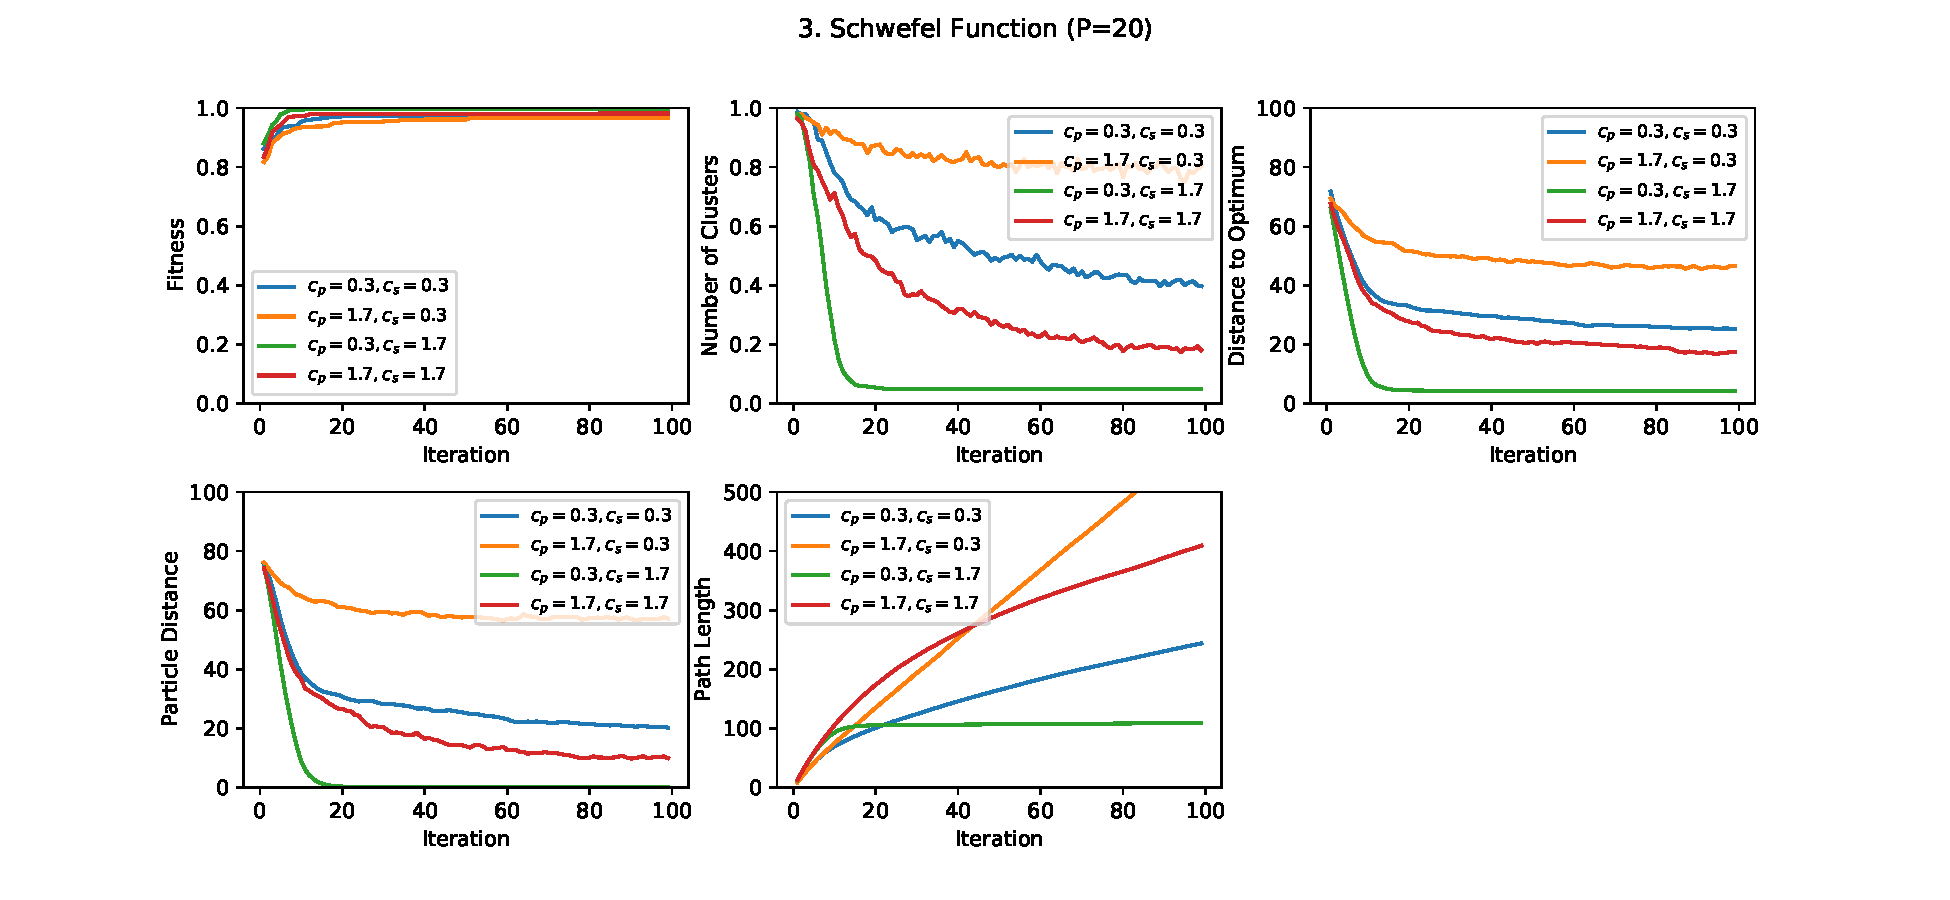
\includegraphics[width=1\textwidth]{figures/ex4/ex4-3-20.pdf}
	\caption{Metrics for Schwefel function and $P=20$}
	\label{fig:ex4-3-20}
\end{figure}
\begin{figure}[h!]
	\centering
	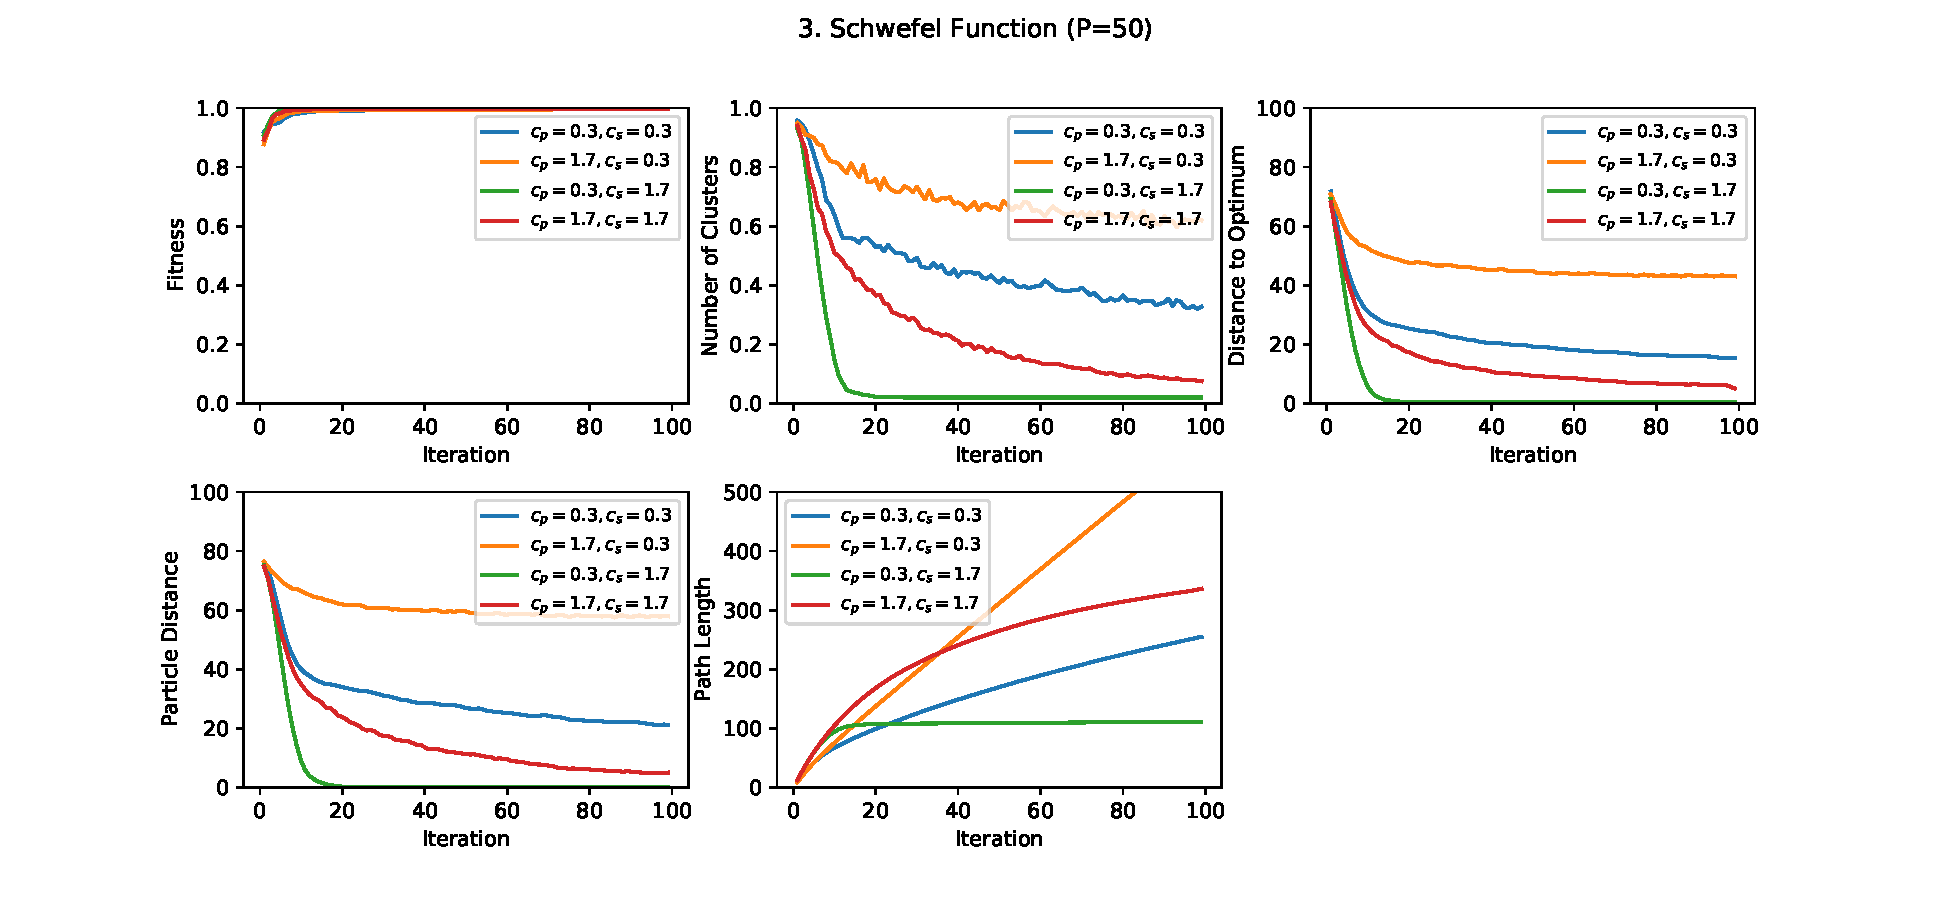
\includegraphics[width=1\textwidth]{figures/ex4/ex4-3-50.pdf}
	\caption{Metrics for Schwefel function and $P=50$}
	\label{fig:ex4-3-50}
\end{figure}

\begin{figure}
\begin{subfigure}[c]{0.5\textwidth}
\centering
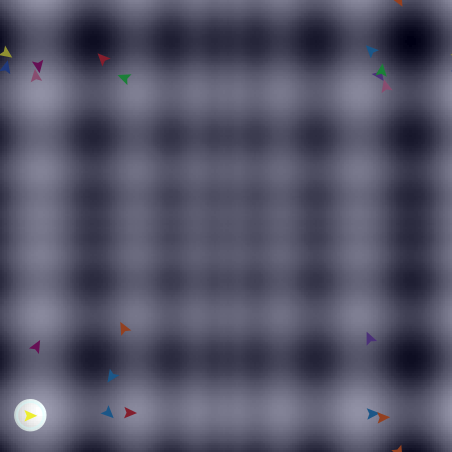
\includegraphics[width=0.75\textwidth]{figures/ex4/ex4-03-17-f3.png}
\subcaption{$c_s=0.3$, $c_p=1.7$}
\label{fig:ex4-example-a}
\end{subfigure}
\begin{subfigure}[c]{0.5\textwidth}
\centering
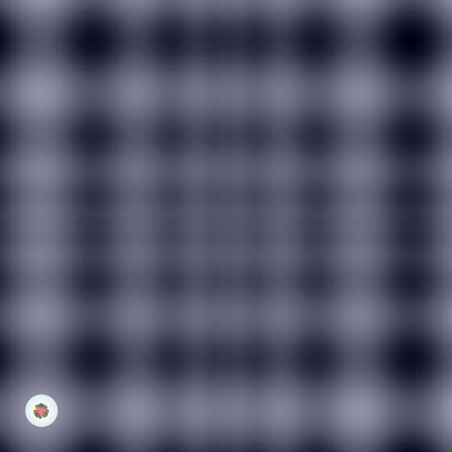
\includegraphics[width=0.75\textwidth]{figures/ex4/ex4-17-03-f3.png}
\subcaption{$c_s=1.7$, $c_p=0.3$}
\label{fig:ex4-example-b}
\end{subfigure}

\caption{Comparison of representative solutions for fitness function $1$ ($P=100$) and $3$ ($P=20$).}
\label{fig:ex4-example}

\end{figure}


\subsection{Inertia}

\begin{figure}
	\centering
	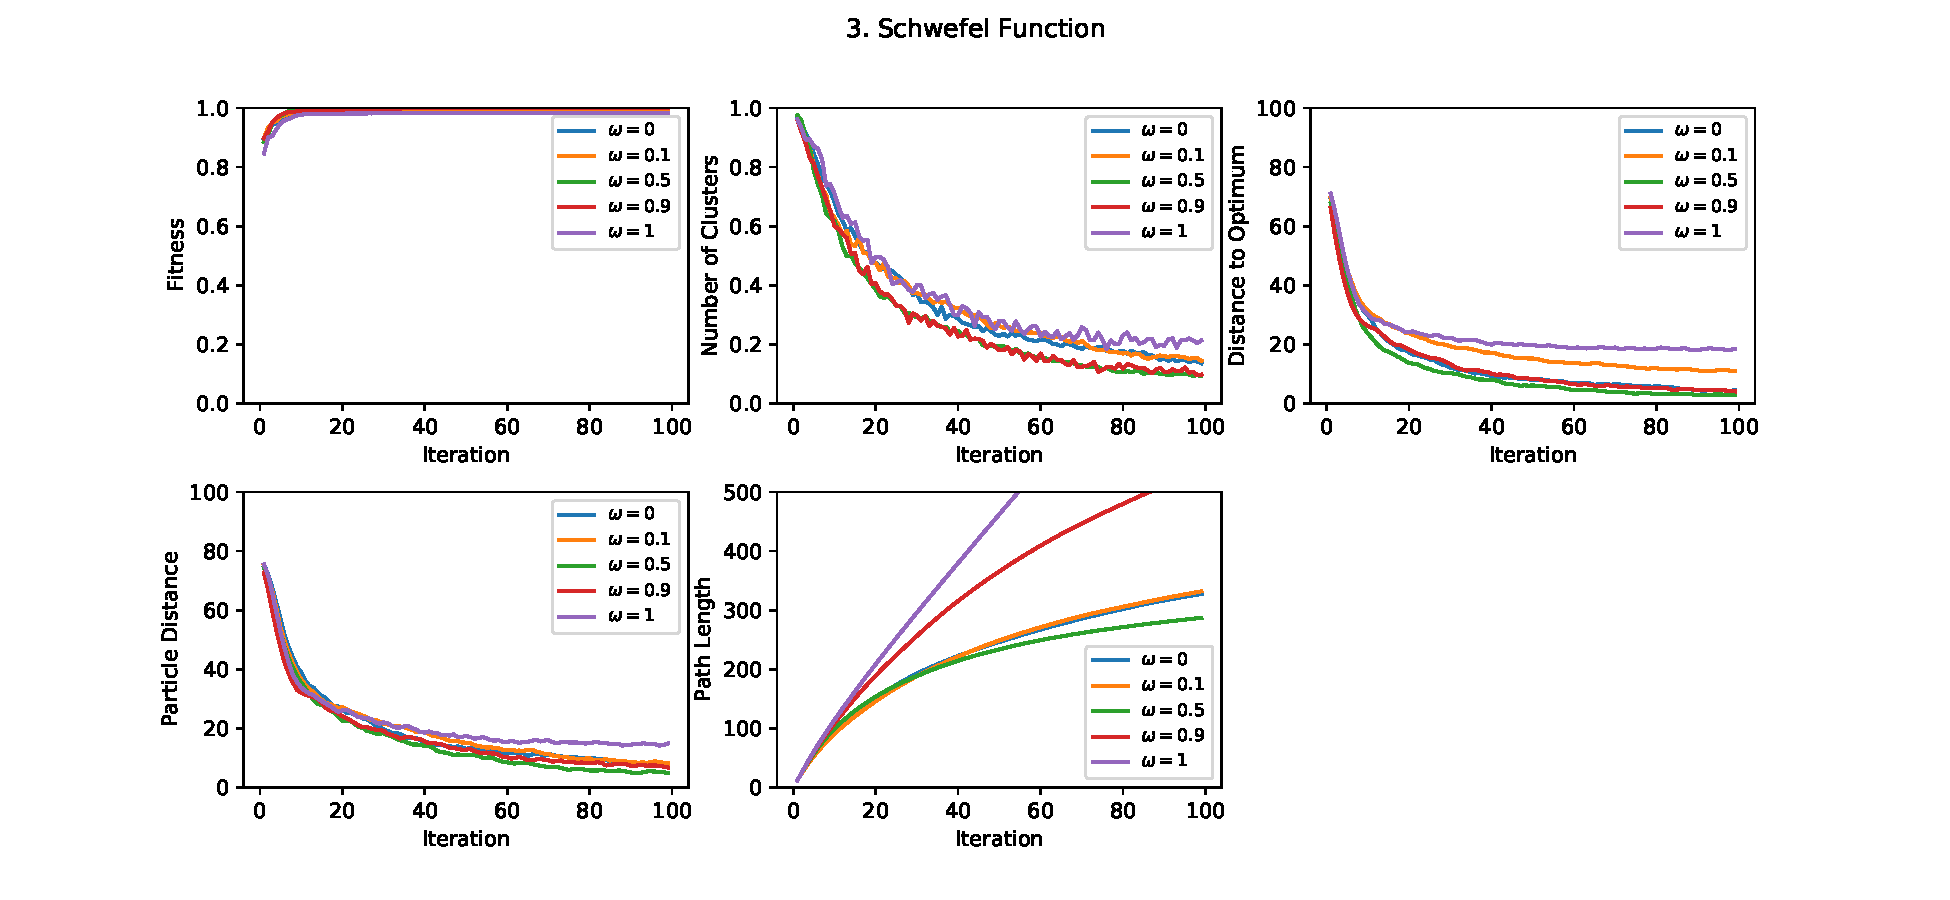
\includegraphics[width=0.9\textwidth]{figures/ex3/ex3-3.pdf}
	\label{fig:ex3-3}
\end{figure}


optimal solution found easily but some 

longer ways, slower convergence of clusters and distance to optimum as well as 

\subsection{Speed Limit}
\begin{figure}
	\centering
	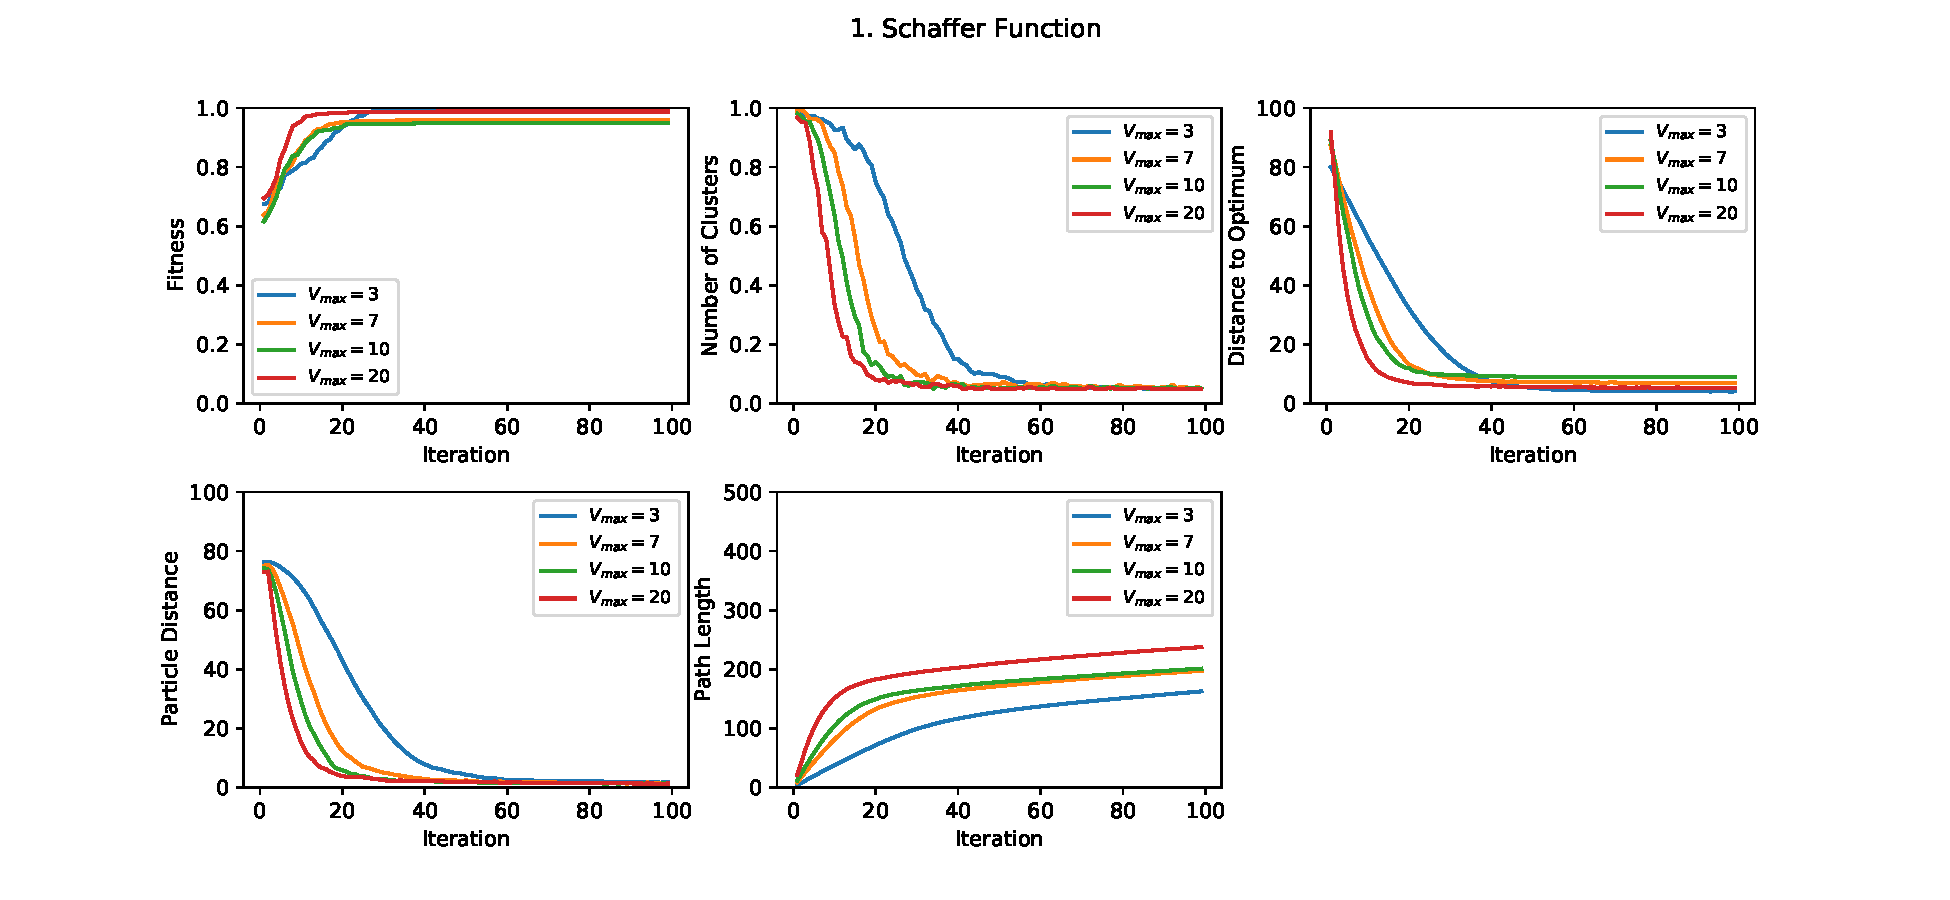
\includegraphics[width=1\textwidth]{figures/ex5/ex5-1.pdf}
	\label{fig:ex5-1}
\end{figure}
\begin{figure}
	\centering
	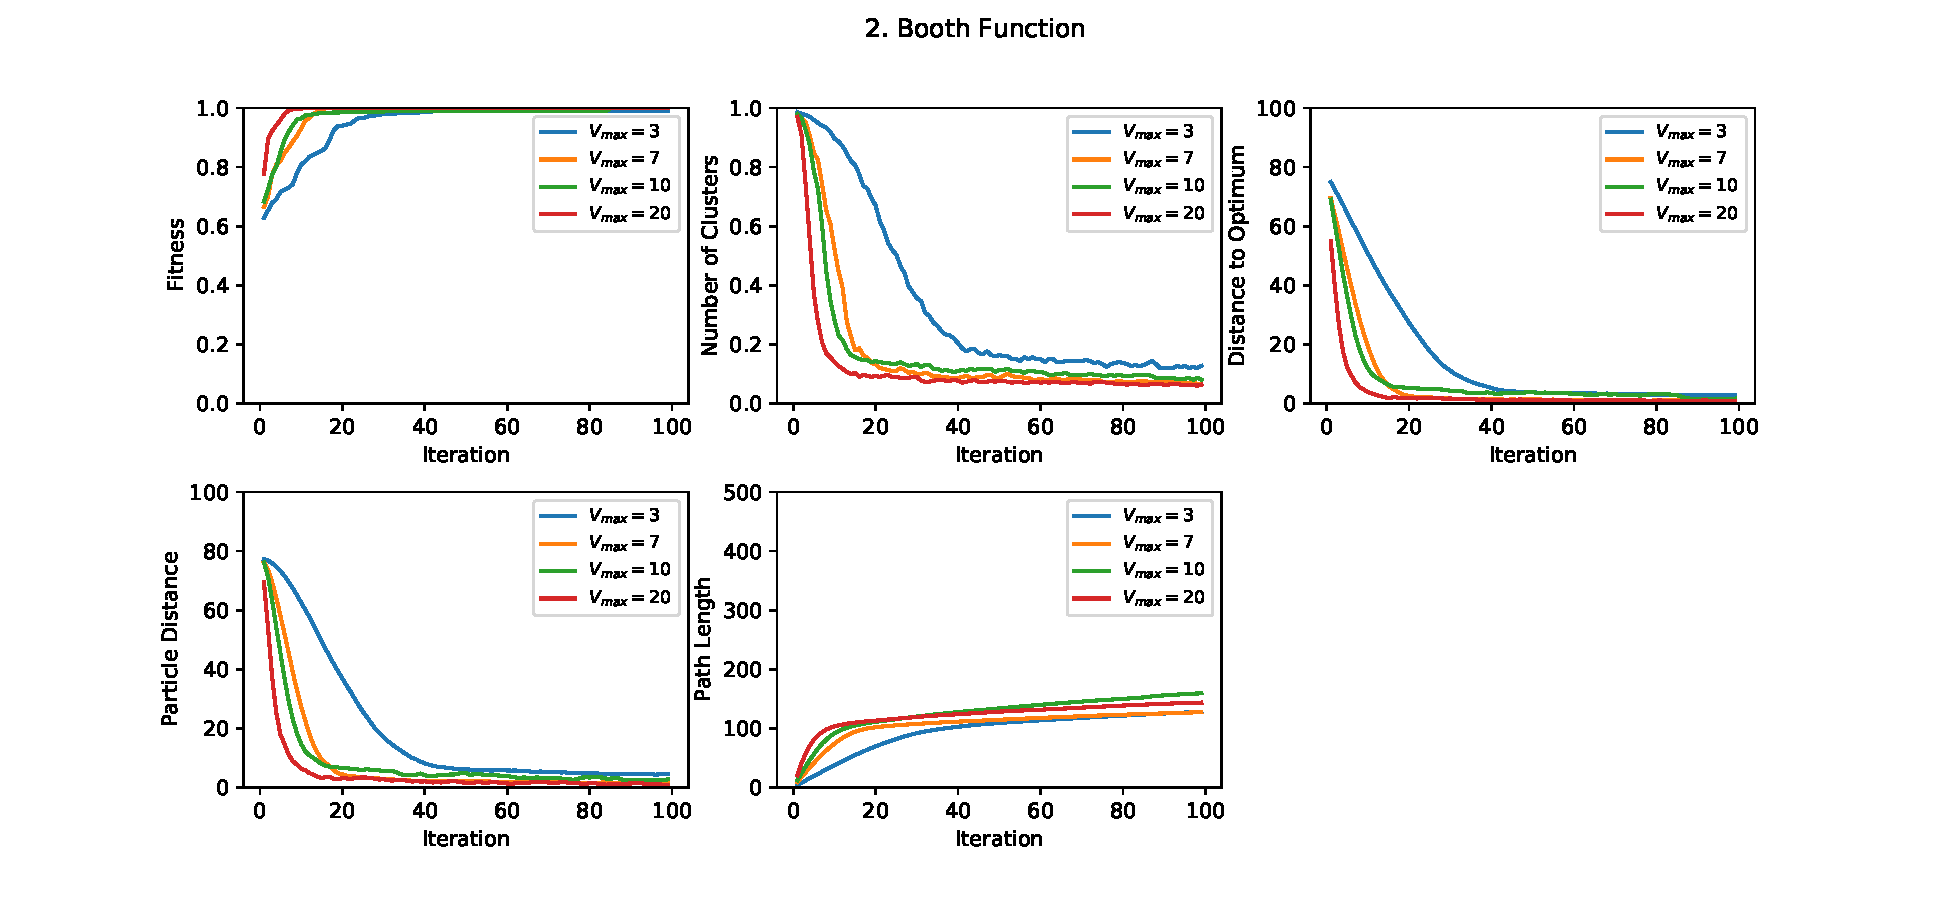
\includegraphics[width=1\textwidth]{figures/ex5/ex5-2.pdf}
	\label{fig:ex5-2}
\end{figure}
\begin{figure}
	\centering
	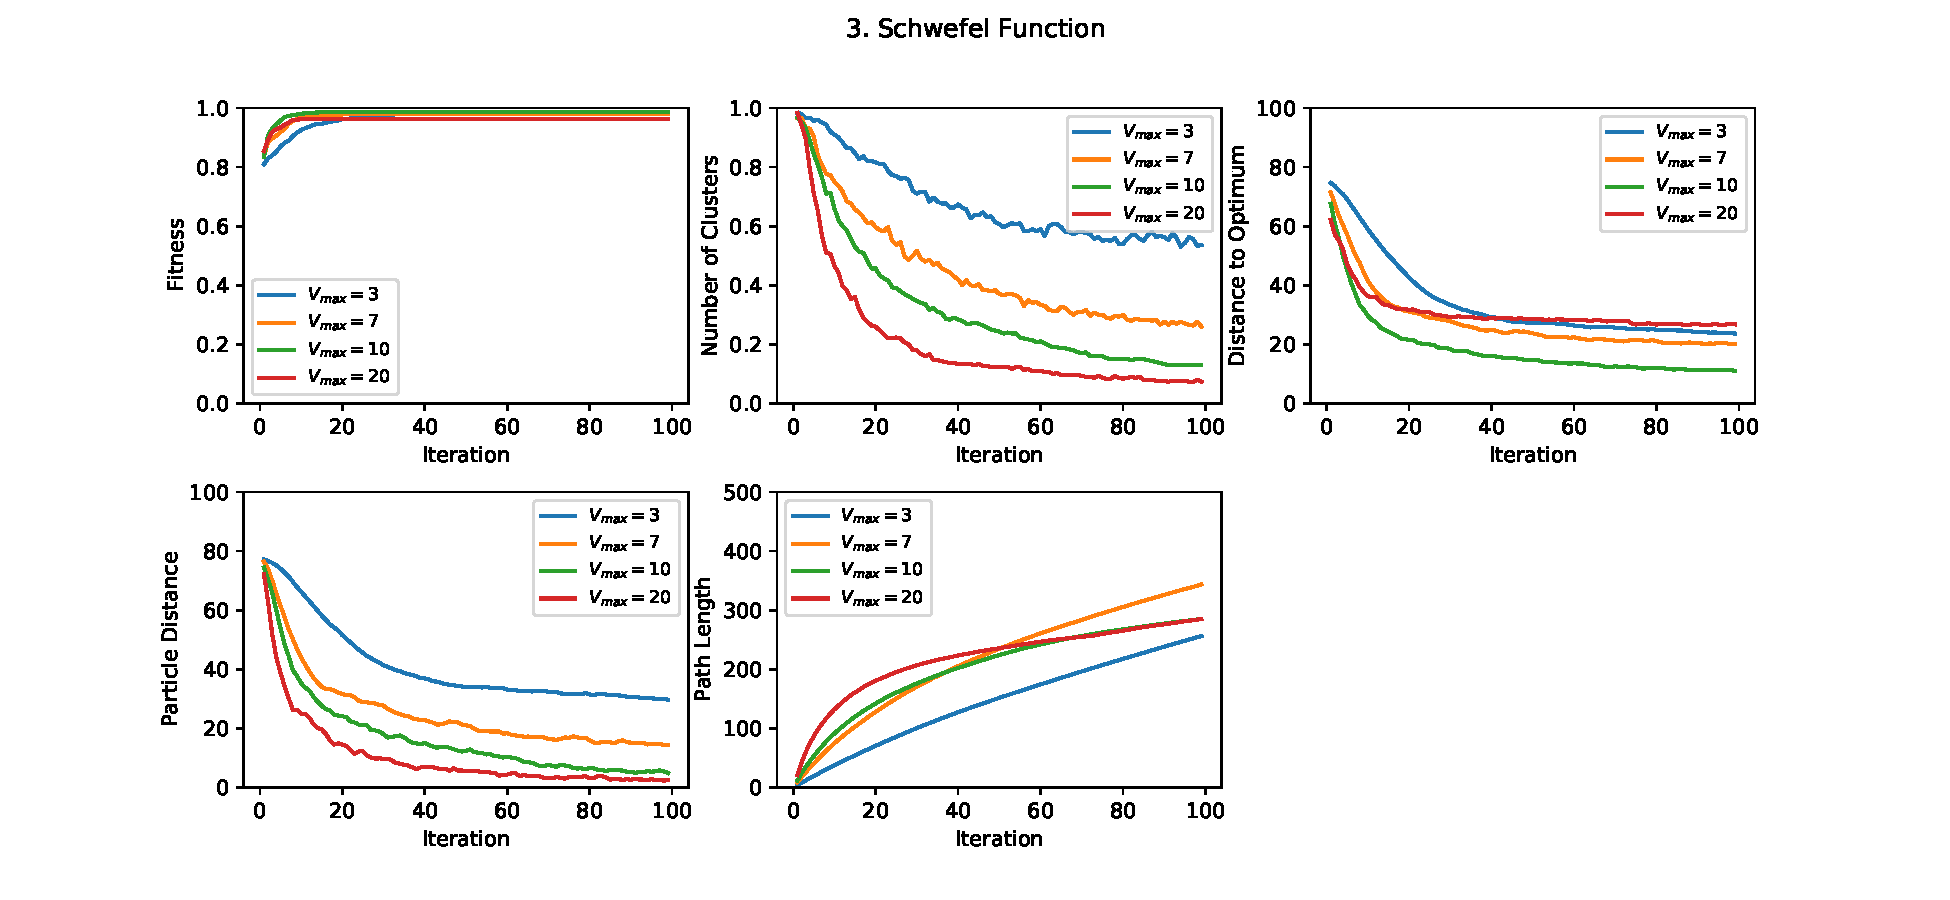
\includegraphics[width=1\textwidth]{figures/ex5/ex5-3.pdf}
	\label{fig:ex5-3}
\end{figure}


\begin{figure}
\begin{subfigure}[c]{0.5\textwidth}
\centering
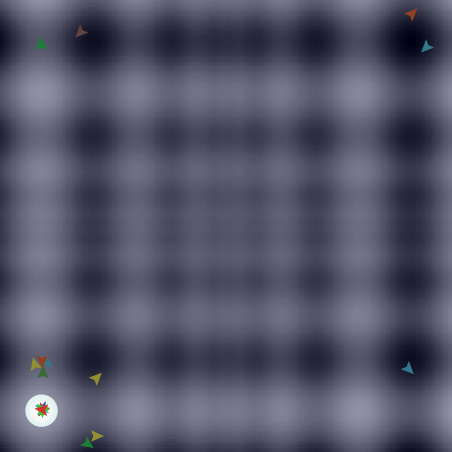
\includegraphics[width=0.75\textwidth]{figures/ex5/f3-3.png}
\subcaption{$V_{max}=3$}
\end{subfigure}
\begin{subfigure}[c]{0.5\textwidth}
\centering
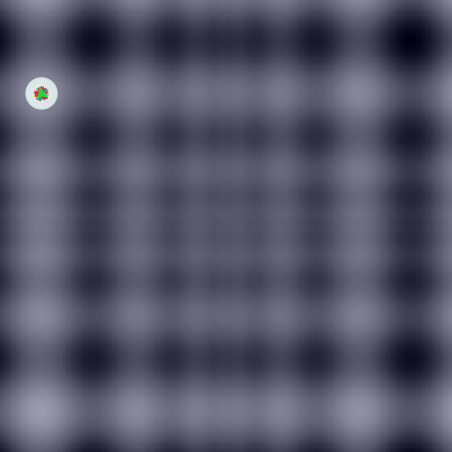
\includegraphics[width=0.75\textwidth]{figures/ex5/f3-20.png}
\subcaption{$V_{max}=20$}
\end{subfigure}

\caption{Comparison of representative solutions for fitness function $1$ ($P=100$) and $3$ ($P=20$).}

\end{figure}


\section{Conclusion}



\bibliographystyle{abbrv}
\bibliography{main}


\end{document}
  